%\title{LaTeX Portrait Poster Template}
%%%%%%%%%%%%%%%%%%%%%%%%%%%%%%%%%%%%%%%%%
% a0poster Portrait Poster
% LaTeX Template
% Version 1.0 (22/06/13)
%
% The a0poster class was created by:
% Gerlinde Kettl and Matthias Weiser (tex@kettl.de)
% 
% Adapter by Jens Buysse for Hogeschool Gent
% This template has been downloaded from:
% http://www.LaTeXTemplates.com
%
% License:
% CC BY-NC-SA 3.0 (http://creativecommons.org/licenses/by-nc-sa/3.0/)
%
%%%%%%%%%%%%%%%%%%%%%%%%%%%%%%%%%%%%%%%%%

%----------------------------------------------------------------------------------------
%	PACKAGES AND OTHER DOCUMENT CONFIGURATIONS
%----------------------------------------------------------------------------------------

\documentclass[a0,portrait]{a0poster}

\usepackage{multicol} % This is so we can have multiple columns of text side-by-side
\columnsep=100pt % This is the amount of white space between the columns in the poster
\columnseprule=3pt % This is the thickness of the black line between the columns in the poster

\usepackage[svgnames]{xcolor} % Specify colors by their 'svgnames', for a full list of all colors available see here: http://www.latextemplates.com/svgnames-colors

\usepackage{times} % Use the times font
%\usepackage{palatino} % Uncomment to use the Palatino font

\usepackage{graphicx} % Required for including images
\graphicspath{{figures/}} % Location of the graphics files
\usepackage{booktabs} % Top and bottom rules for table
\usepackage[font=small,labelfont=bf]{caption} % Required for specifying captions to tables and figures
\usepackage{amsfonts, amsmath, amsthm, amssymb} % For math fonts, symbols and environments
\usepackage{wrapfig} % Allows wrapping text around tables and figures
\usepackage[export]{adjustbox}

\begin{document}

%----------------------------------------------------------------------------------------
%	POSTER HEADER 
%----------------------------------------------------------------------------------------

% The header is divided into two boxes:
% The first is 75% wide and houses the title, subtitle, names, university/organization and contact information
% The second is 25% wide and houses a logo for your university/organization or a photo of you
% The widths of these boxes can be easily edited to accommodate your content as you see fit

\begin{minipage}[t]{0.75\linewidth}
\VeryHuge \color{HoGentAccent1} \textbf{Open source serverless infrastructuur} \color{Black}\\ % Title
\Huge\textit{Onderzoek naar serverless computing en open source serverless infrastructuur: vergelijkende studie en Proof of Concept}\\[2.4cm] % Subtitle
\huge \textbf{Mertens Lennert, Saveyn Pieter-Jan, Van Impe Steven}\\[0.5cm] % Author(s)
\huge Hogeschool Gent, Valentin Vaerwyckweg 1, 9000 Gent\\[0.4cm] % University/organization
\Large \texttt{lennert.mertens@student.hogent.be} \\
\end{minipage}
%
\begin{minipage}[t]{0.25\linewidth}

\includegraphics[width=13cm,right]{figures/HOGENT_Logo_Pos_rgb.png} 

\end{minipage}

\vspace{1cm} % A bit of extra whitespace between the header and poster content

%----------------------------------------------------------------------------------------

\begin{multicols}{2} % This is how many columns your poster will be broken into, a portrait poster is generally split into 2 columns

%----------------------------------------------------------------------------------------
%	ABSTRACT
%----------------------------------------------------------------------------------------

\color{HoGentAccent1} % Navy color for the abstract

\begin{abstract}
Serverless computing is een ''hot topic'' en kent een grote opmars binnen de IT wereld. Verschillende bedrijven hebben deze technologie reeds geadopteerd en in de toekomst zullen er nog heel veel volgen. Omdat de strijd binnen de serverless wereld nog niet gestreden is en er nog geen standaard is gezet, is een onderzoek naar veelbelovende open source serverless oplossingen zinvol. Nubera is op zoek naar een open source serverless framework, dat aanleunt bij hun requirements, om aan te bieden bij klanten die serverless willen gaan werken. Nubera gaf aan interesse te hebben in Fission en zocht hiervoor een veelbelovend alternatief. Dit onderzoek vergelijkt Fission met OpenFaaS, een zelfgekozen framework conform vooropgestelde requirements.
\end{abstract}
%----------------------------------------------------------------------------------------
%	INTRODUCTION
%----------------------------------------------------------------------------------------
\color{HoGentAccent1} 
\section*{Introductie}
\color{black}
\color{black}
De jongste jaren is er een nieuwe trend in Cloud computing geëvolueerd, namelijk serverless of vaak gerefereerd als Function-as-a-Service. Serverless technologie biedt heel wat voordelen op basis van verschillende aspecten. Het voornaamste voordeel van serverless computing is dat het overhead, omtrent beheer van infrastructuur, wegneemt bij softwareontwikkelaars en hun instaat stelt enkel te focussen op wat er voor hen het meest toe doet, namelijk de softwareontwikkeling zelf.
Deze studie behandelt een uiteenzetting van de cloud computing basisprincipes zoals de verschillen tussen verschillende service niveaus in figuur 1. Er wordt ook onderzoek gedaan naar wat serverless concreet inhoudt, wat de voor- en nadelen zijn en welke componenten serverless mogelijk maken. Daarnaast wordt op basis van verschillende requirements een overweging gemaakt voor het kiezen van een open source Kubernetes native framework dat de mogelijkheden aanbiedt om serverless te draaien in house (in een eigen datacenter of private cloudomgeving). Het onderzoek wordt gestaafd met een Proof of Concept die twee frameworks vergelijkt, enerzijds Fission, dat werd aangereikt door Nubera en anderzijds een alternatief dat op basis van requirements wordt gekozen, namelijk OpenFaaS.
\\
\begin{center}\vspace{1cm}
    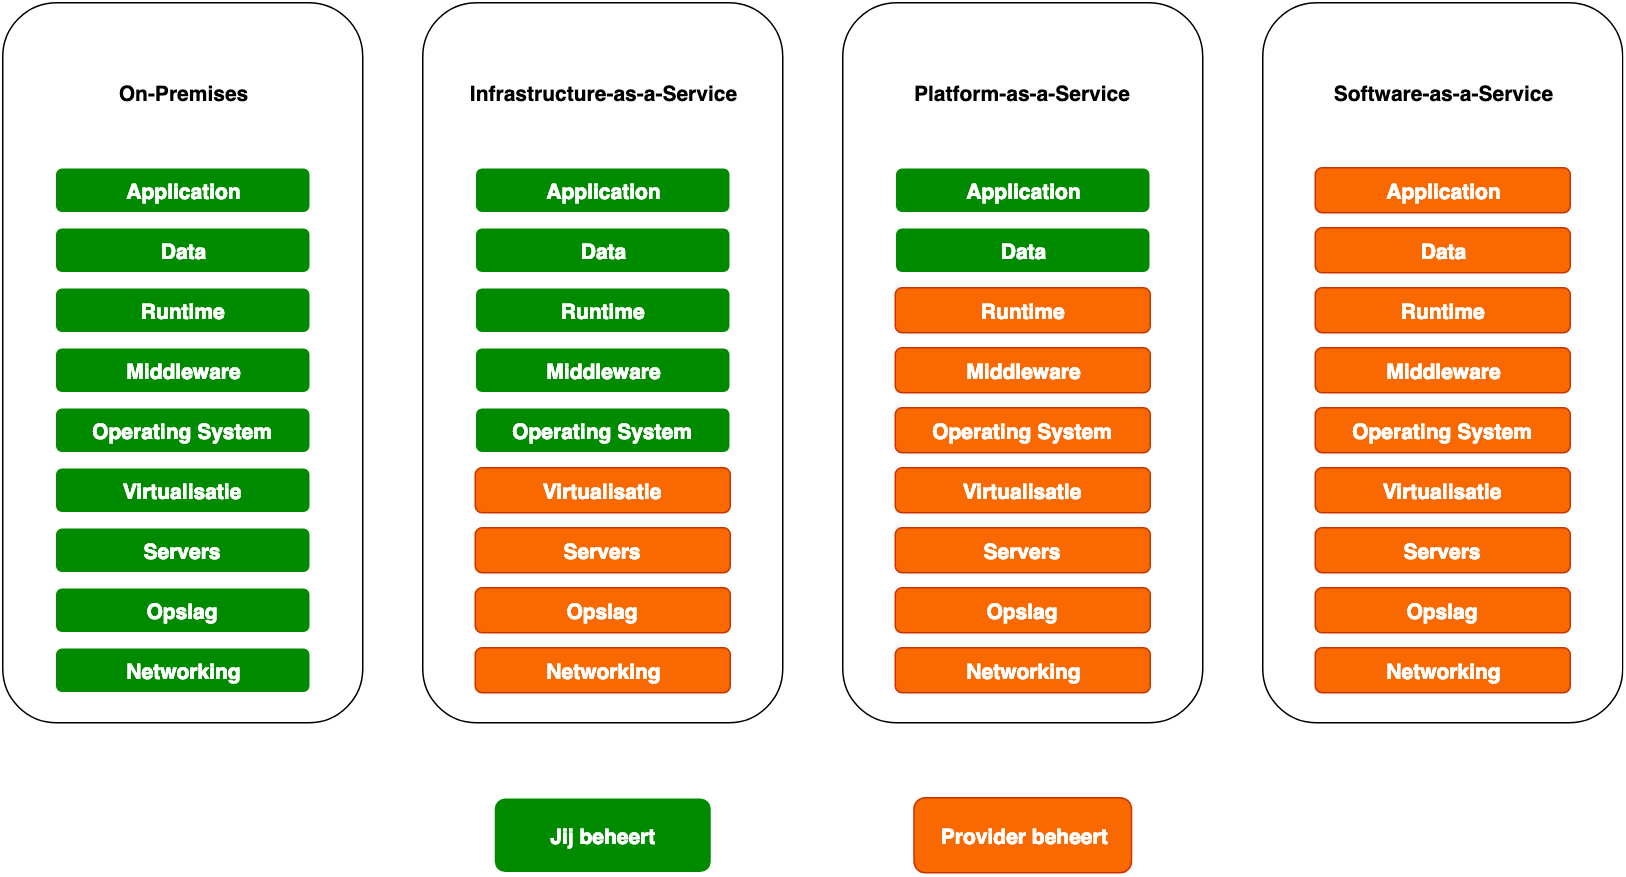
\includegraphics[width=0.8\linewidth]{service-niveaus}
    \label{fig:service-niveaus}
    \captionof{figure}{\color{HoGentAccent5} Cloud service niveaus.}
\end{center}\vspace{1cm}
%----------------------------------------------------------------------------------------
%	GEOLOGY
%----------------------------------------------------------------------------------------

\color{Black} % DarkSlateGray color for the rest of the content
\color{HoGentAccent1} 
\section*{Experimenten}
\color{black}
In overleg met Nubera werden requirements gecapteerd waaraan de frameworks moeten voldoen. Fission en OpenFaaS worden tegenover elkaar afgewogen op basis van deze requirements. Sommige vereisten kunnen worden vergeleken aan de hand van literair onderzoek, voor anderen is een uitwerking nodig met behulp van een Proof of Concept. 
Sommige zaken, die worden behandeld in het onderzoek, worden beoordeeld op basis van persoonlijke voorkeur zoals het meest gebruiksvriendelijk en dergelijke, doch worden deze meningen sterk onderbouwt, zodat lezers kunnen aannemen waarom dit zo is. De Proof of Concept vergelijkt beide frameworks op analoge manier, alle stappen die bij het ene framework aan bod komen, zijn ook terug te vinden bij het andere. Alvorens de frameworks worden getest werd er een Python demofunctie geschreven die dient ter illustratie en inzicht geeft in hoe de frameworks functioneren.
\\\\
Fission en OpenFaaS worden tegenover elkaar afgewogen op basis van verschillende vereisten:
\begin{itemize}
    \item Eenvoud van installatie.
    \item Deployment en uitvoeringstijd van functies.
    \item Gebruik van command line tools en User Interface.
    \item Monitoring.\\
\end{itemize}

Een gedetailleerd overzicht in de verschillen tussen de frameworks is terug te vinden in de Proof of Concept van dit onderzoek. De resultaten worden echter wel reeds kort en bondig besproken in de conclusie.
\\\\\\\\\\\\\\
\color{HoGentAccent1} 
\section*{Metingen}
\color{black}
Om inzicht te krijgen in de snelheid van de frameworks werden beide getest aan de hand van, enerzijds de zelfgeschreven Python functie, anderzijds een simpele ''Hello World'' Python functie. De uitvoeringstijd van de zelfgeschreven functie bij Fission ligt een stukje lager in vergelijking met OpenFaaS. 

\begin{center}\vspace{1cm}
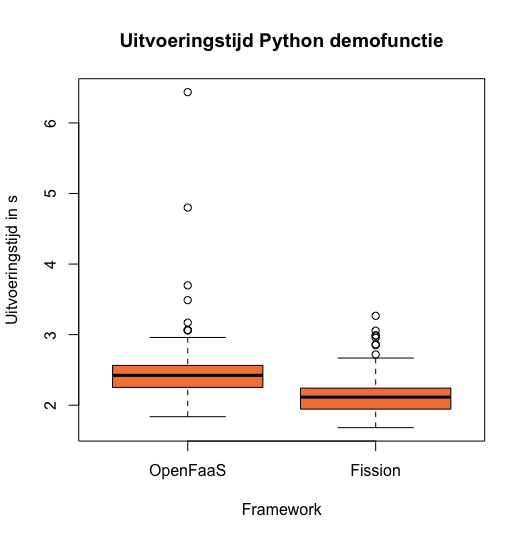
\includegraphics[width=0.5\linewidth]{boxplot-uitvoeringstijd-demofunctie}
\captionof{figure}{\color{HoGentAccent5} Uitvoeringstijd zelfgeschreven Python demofunctie.}
\end{center}\vspace{1cm}

 Wanneer er een extra vergelijking wordt gemaakt met een simpele ''Hello World'' functie, dan blijkt hier ook Fission heel wat sneller te zijn. Het is duidelijk dat wanneer uitvoeringssnelheid primeert, Fission het meest interessante framework zal zijn. Het verschil in gebruik is nauwelijks merkbaar maar op basis van de cijfers is te zien dat dit toch wel aanzienlijk is.
 
\begin{center}\vspace{1cm}
    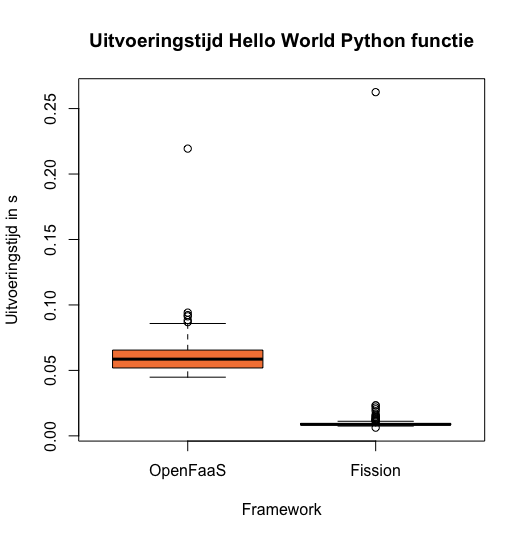
\includegraphics[width=0.5\linewidth]{boxplot-uitvoeringstijd-hellofunctie}
    \captionof{figure}{\color{HoGentAccent5} Uitvoeringstijd ''Hello World'' Python functie.}
\end{center}\vspace{1cm}



%------------------------------------------------



\color{HoGentAccent1} 
\section*{Conclusies}
\color{black}
Uit de experimenten blijkt het ene framework beter te scoren dan het andere. Fission blijkt beter te presteren op basis van executietijd. De demofuncties die op het Fission framework werden gedeployed en aangeroepen hebben een kortere uitvoeringstijd dan de functies op OpenFaaS. OpenFaaS daarentegen biedt de aangenaamste gebruikerservaring voor gebruikers die nieuw zijn in serverless computing. De UI die OpenFaaS standaard meelevert in de installatie is eveneens gebruiksvriendelijk en eenvoudig in gebruik. De interface is intuïtief en vereist geen ervaring met OpenFaaS. OpenFaaS voorziet in tegenstelling tot Fission wel YAML templating voor het definiëren van functies. Bij het uitwerken van de Proof of Concept verliep alles vlotter en sneller bij OpenFaaS, dit is te danken aan de verschillende bronnen die hierover terug te vinden zijn en de duidelijke documentatie die beschikbaar is. In het onderzoek werd getracht het meest interessante open source serverless framework in overeenstemming met de vereisten van Nubera te vinden. Op basis van literair onderzoek, uitgevoerde experimenten en resultatenverwerking werd er tot een besluit gekomen. Het meest veelbelovende framework voor Nubera, op moment van schrijven, is OpenFaaS.

%----------------------------------------------------------------------------------------
%	FORTHCOMING RESEARCH
%----------------------------------------------------------------------------------------
\color{HoGentAccent1} 
\section*{Toekomstig onderzoek}
\color{black}
Er werden twee veelbelovende open source Kubernetes native serverless frameworks behandeld, maar er bestaan nog alternatieven die verder onderzoek meer dan waard zijn. Hopelijk kan deze bachelorproef een aanzet geven voor verder onderzoek naar andere, misschien minder bekende maar veelbelovende, open source serverless frameworks. Het zou interessant zijn dat dit document wordt uitgebreid met extra frameworks, zo kan dit onderzoek inzicht geven in alle mogelijke Kubernetes native serverless frameworks en deze tegenover elkaar afwegen.
%----------------------------------------------------------------------------------------
\end{multicols}
\end{document}